\chapter{Quantum-dot cellular automata}

\graphicspath{{../gfx/chapter01/}}

\begin{figure}
  \center
  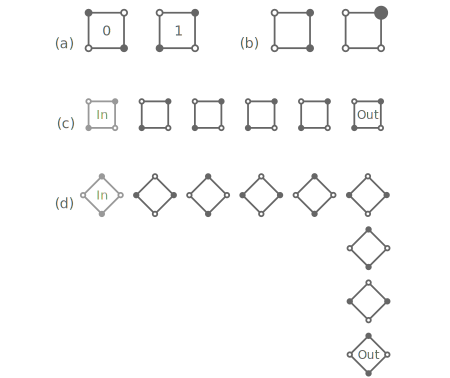
\includegraphics{intro_qca}
  \caption{\ldots}
  \label{fig:intro_qca}
\end{figure}

Lent et al.\ introduced the concept of quantum-dot cellular automata as an
alternative computing paradigm in 1993 \cite{lent1993quantum}. Thus the aim was
a novel physical scheme to build digital circuits that would overcome some of
the limitations of CMOS technology, promising potentially lower power
consumption, higher device density, and faster clocking. As the name alludes to,
quantum-dot cellular automata (QCA) is built from quantum-dots which are grouped
together in cells. Figure~\ref{fig:intro_qca}(a) shows a basic QCA cell. Four
quantum dots are arranged on the corners of a square. The dots are idealized as
perfectly localized single orbitals on a perfectly decoupled non-intrusive
medium. Therefore, each dot can be occupied by up to two electrons. In the QCA
scheme, however, each cell is occupied by only two electrons in total. The cell
is quarter-filled. The electrons tunnel between different dots in a cell, but
the dominant energy scale is set by the Coulomb repulsion between the particles.
Simply by virtue of the Coulomb repulsion, and ignoring the comparatively small
tunnelling for now, the diagonal states, Fig.~\ref{fig:intro_qca}(a), are the
two energetically preferred electron configurations. In comparison, edge states
or doubly occupied quantum dots are unfavourable higher energy states,
Fig.~\ref{fig:intro_qca}(b). A priori the two diagonal states are energetically
degenerate, but this degeneracy can be lifted by introducing an external Coulomb
potential, for example a second nearby QCA cell. Then these two states can be
identified with logic 0 and 1, as indicated in the figure.

A single cell by itself is, of course, not very interesting. Thus, multiple
cells can be positioned next to each other, for example as a straight line of
cells, Fig.\ref{fig:intro_qca}(c). The approach now again assumes that Coulomb
is the driving force and that electron tunnelling between cells is very small
and ideally zero. For a straight line of cells, these long-ranging, unscreened
Coulomb forces will tend to align the electron configurations of adjacent cells.
If the first cell is in logic state 1 then the second cell will also prefer
logic state 1 and so will in turn all the other cells in the line. The situation
is the same for logic state 0. Therefore, a straight line of cells is similar to
a wire not only in geometry, but also in functionality: It transmits a digital
signal. The same is true, with slight modifications, for a diagonal line of
cells --- cells rotated by $45^{\circ}$---, Fig.~\ref{fig:intro_qca}(d). In this
case the signal alternates from cell to cell, that is, logic 1 will follow logic
0 which followed from logic 0, and this again is simply by virtue of the
dominant Coulomb interactions between electrons on different cells. By using an
even number of cells the diagonal line of cells works as a wire just as well as
a straight line of cells. The pictogram also demonstrates a $90^{\circ}$ for the
diagonal line of cells which our newly gained intuition for these Coulomb-driven
systems expects to pose no problem for signal transmission.

The main idea of the QCA approach becomes apparent: Ideally bistable cells
interact with each other solely by Coulomb repulsion. By arranging the cells in
clever geometries we can realize interesting functionalities. One such clever
geometrical arrangement is the majority gate, Fig.~\ref{fig:intro_qca}(e). The
gate has three inputs which ``vote'' on the central cell. The majority wins and
sets the single output. The device is commonly operated with one fixed input,
for example $I_3 \doteq 0$ or $I_3 \doteq 1$. In the first case, $I_3 \doteq 0$,
the device functions as an AND gate for the remaining two inputs, $O = I_1 \land
I_2$. In the second case, $I_3 \doteq 1$, it is an OR gate with $O = I_1 \lor
I_2$. Now, the only missing piece for Boolean algebra is negation, $O = \lnot
I$. We had already seen that simply arranging cells at an $45^{\circ}$ angle as
in the diagonal line of cells above negates the signal from cell to cell. The
inverter, Fig.~\ref{fig:intro_qca}(f) recasts this idea into a more robust
layout. With that we have, at least in principle, all the necessary building
blocks for Boolean algebra and thus digital circuitry.

Let us note that QCA is a not a cellular automata in a strict mathematical sense,
but only by analogy to the idea of interacting cells.



